\documentclass[10pt]{scrartcl}

\usepackage[utf8]{inputenc}
\usepackage{tabularx}
\usepackage{longtable}
\usepackage[ngerman]{babel}
\usepackage[automark]{scrpage2}
\usepackage{amsmath,amssymb,amstext}
\usepackage[]{color}
\usepackage[]{enumerate}
\usepackage{graphicx}
\usepackage{polynom}
\usepackage{lastpage}
\usepackage[perpage,para,symbol*]{footmisc}
\usepackage{listings} 
\usepackage[pdfborder={0 0 0},colorlinks=false]{hyperref}
\usepackage[numbers,square]{natbib}
\usepackage{color}
\usepackage{colortbl}
\usepackage[absolute]{textpos}
\usepackage{float}
\usepackage[colorinlistoftodos,textsize=small,textwidth=2cm,shadow,bordercolor=black,backgroundcolor={red!100!green!33},linecolor=black]{todonotes}

\lstset{numbers=left, numberstyle=\tiny, numbersep=5pt, breaklines=true, showstringspaces=false} 
\restylefloat{figure}

%changehere
\def\titletext{Uebungsblatt 1}
\def\titletextshort{Praktikum 1}
\author{André Harms, Oliver Steenbuck}

\title{\titletext}

%changehere Datum der Übung
\date{19.04.2012}

\pagestyle{scrheadings}
%changehere
\ihead{TH1, Padberg}
\ifoot{Generiert am:\\ \today}

\cfoot{Oliver Steenbuck, André Harms}


\ohead[]{\titletextshort}
\ofoot[]{{\thepage} / \pageref{LastPage}}

\setlength{\parindent}{0.0in}
\setlength{\parskip}{0.1in}

\begin{document}
\maketitle

\setcounter{tocdepth}{3}
\tableofcontents

%	\listoftables                                 												% 
	\listoffigures  
	\lstlistoflistings	

\section{Aufgabe 1}
	\subsection{Formale Definition des Netzes}
	\begin{align}
	&N =\{P,T,W,M_0\}\\
	&P =\{p1,p2,p3,p4\}\\
	&T =\{t1,t2,t3\}\\
	&W(x,y) =\begin{cases}
			2 \text{ ;falls } (x,y) \in \{(t1,p2),(t2,p3)\} \\
			1 \text{ ;falls } (x,y) \in \{(p1,t1),(p2,t2), (p3,t3), (t3,p1), (t3,p4)\} \\
			0 \text{ ;sonst}
	     \end{cases}\\
	&M_0(x)=  \begin{cases}
			1 \text{ ;falls } x=p1\\
			0 \text{ ;sonst}
	     \end{cases}   
	\end{align}	

	\subsection{Schalthäufigkeit}
	Das Netz kann beliebig oft schalten.

\section{Aufgabe 2}
	\subsection{Formale Definition des Netzes}
	\begin{align}
	&N =\{P,T,W,M_0\}\\
	&P =\{p1,p2,p3,p4\}\\
	&T =\{t1,t2,t3\}\\
	&W(x,y) =\begin{cases}
			2 \text{ ;falls } (x,y) \in \{(t1,p2),(t2,p3)\} \\
			1 \text{ ;falls } (x,y) \in \{(p1,t1),(p2,t2), (p3,t3), (t3,p1), (t3,p4)\} \\
			0 \text{ ;sonst}
	     \end{cases}\\
	&M_0(x)=  \begin{cases}
			1 \text{ ;falls } x=p1\\
			0 \text{ ;sonst}
	     \end{cases}\\  
	&K(x)=  \begin{cases}
			7 \text{ ;falls } x=p1\\
			4 \text{ ;falls } x=p4\\
			\omega \text{ ;sonst}
	     \end{cases} 
	\end{align}	
	
	\subsection{Schalthäufigkeit}
	Nein, da durch die Kapazität auf $p4$ die Transition $t3$ maximal 4 mal geschaltet werden kann und $p1$ diese Transition benötigt. 

\section{Aufgabe 3}
\subsection{Formale Definition des Netzes}
	\begin{align}
	&N =\{P,T,F,M_0\}\\
	&P =\{p1,p2,p3\}\\
	&T =\{t1,t2,t3\}\\
	&F(x,y) =\begin{cases}
			1 \text{ ;falls } (x,y) \in \{(p1,t1),(t1,p2),(t1,p3),(p2,t2),(t2,t1),(p3,t3),(t3,p1)\} \\
			0 \text{ ;sonst}
	     \end{cases}\\	
	&M_0(x)=  \begin{cases}
			1 \text{ ;falls } x=p1\\
			0 \text{ ;sonst}
	     \end{cases}        
	\end{align}	
	
	\subsection{Schaltschritte}
	
	\subsubsection{Schaltschritt 1}	
		\begin{align}	
			&t1 \text{ ist M-aktiviert da gilt } p \in \bullet t1:M(p) \geq W(p,t1)\\
			&\text{ genauer }\begin{cases}
				M(p1) \geq W(p1,t1) = 1 \geq 1	
			\end{cases}\\
			&M^{'}(p) \text{ bestimmt sich also durch } M(p) - W(p,t1) + W(t1,p) \text{ für }  p \in P\\
			&\text{ genauer }\begin{cases}
				M^{'}(p1) = M(p1) - W(p1,t1) + W(t1,p1) = 1 - 1 + 0 = 0\\
				M^{'}(p2) = M(p2) - W(p2,t1) + W(t1,p2) = 0 - 0 + 1 = 1\\ 
				M^{'}(p3) = M(p3) - W(p3,t1) + W(t1,p3) = 0 - 0 + 1 = 1\\ 
			\end{cases}\\
			&M\overset{t1}{\rightarrow}M^{'}			
		\end{align}
		
	\subsubsection{Schaltschritt 2}
		\begin{align}	
			&t2 \text{ ist M-aktiviert da gilt } p \in \bullet t2:M(p) \geq W(p,t2)\\
			&\text{ genauer }\begin{cases}
				M(p2) \geq W(p2,t2) = 1 \geq 1	
			\end{cases}\\
			&M^{'}(p) \text{ bestimmt sich also durch } M(p) - W(p,t2) + W(t2,p) \text{ für }  p \in P\\
			&\text{ genauer }\begin{cases}
				M^{'}(p1) = M(p1) - W(p1,t2) + W(t2,p1) = 0 - 0 + 1 = 1\\
				M^{'}(p2) = M(p2) - W(p2,t2) + W(t2,p2) = 1 - 1 + 0 = 0\\ 
				M^{'}(p3) = M(p3) - W(p3,t2) + W(t2,p3) = 1 - 0 + 0 = 1\\ 
			\end{cases}\\
			&M\overset{t2}{\rightarrow}M^{'}			
		\end{align}
		
	\subsection{Konflikte}
	Es besteht ein Rückwärtskonflikt bei $p1$ da die beiden Tansitionen $t2$ und $t3$ nach schalten.
	
\section{Aufgabe 4}
	\subsection{Petrinetz}
	\begin{figure}[H]
    		\centering
			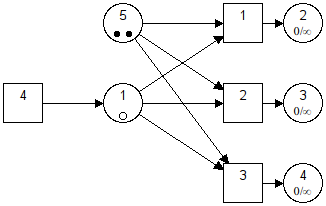
\includegraphics[]{aufg4.png}		
            \caption{Petri Netz Aufgabe 4}
            \label{petri:aufg4}
	\end{figure}
	
	\subsection{Prozessnetze}
		\subsubsection{Prozessnetz 1}
			\begin{figure}[H]
    			\centering
				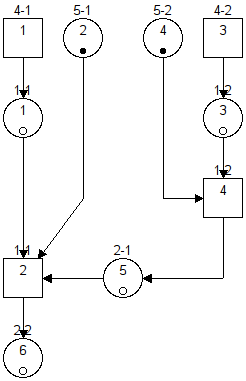
\includegraphics[]{aufg4Proc1.png}		
            	\caption{Petri Netz Aufgabe 4 Prozessnetz 1}
            	\label{petri:aufg4:pro1}
			\end{figure}	

			\begin{figure}[H]
    			\centering
				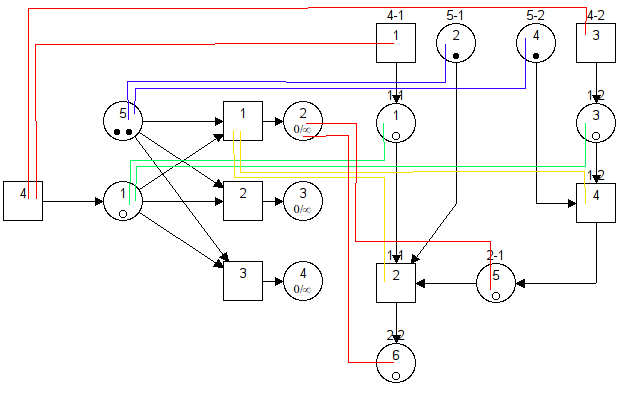
\includegraphics[scale=0.5]{transf1.png}		
            	\caption{Netzmorphismus Aufgabe 4 Prozessnetz 1}
            	\label{petri:aufg4:pro1:morph}
			\end{figure}				
				
		\subsubsection{Prozessnetz 2}
			\begin{figure}[H]
    			\centering
				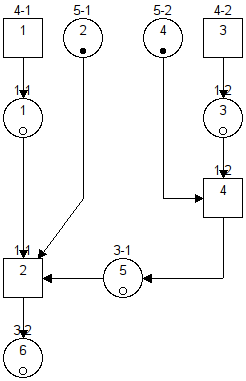
\includegraphics[]{aufg4Proc2.png}		
            	\caption{Petri Netz Aufgabe 4 Prozessnetz 2}
            	\label{petri:aufg4:pro2}
			\end{figure}		
		\subsubsection{Prozessnetz 3}
			\begin{figure}[H]
    			\centering
				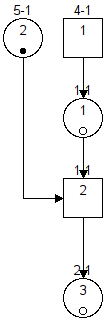
\includegraphics[]{aufg4Proc3.png}		
            	\caption{Petri Netz Aufgabe 4 Prozessnetz 3}
            	\label{petri:aufg4:pro3}
			\end{figure}		

\end{document}

